% Options for packages loaded elsewhere
\PassOptionsToPackage{unicode}{hyperref}
\PassOptionsToPackage{hyphens}{url}
\PassOptionsToPackage{dvipsnames,svgnames,x11names}{xcolor}
%
\documentclass[
  letterpaper,
  DIV=11,
  numbers=noendperiod]{scrartcl}

\usepackage{amsmath,amssymb}
\usepackage{iftex}
\ifPDFTeX
  \usepackage[T1]{fontenc}
  \usepackage[utf8]{inputenc}
  \usepackage{textcomp} % provide euro and other symbols
\else % if luatex or xetex
  \usepackage{unicode-math}
  \defaultfontfeatures{Scale=MatchLowercase}
  \defaultfontfeatures[\rmfamily]{Ligatures=TeX,Scale=1}
\fi
\usepackage{lmodern}
\ifPDFTeX\else  
    % xetex/luatex font selection
\fi
% Use upquote if available, for straight quotes in verbatim environments
\IfFileExists{upquote.sty}{\usepackage{upquote}}{}
\IfFileExists{microtype.sty}{% use microtype if available
  \usepackage[]{microtype}
  \UseMicrotypeSet[protrusion]{basicmath} % disable protrusion for tt fonts
}{}
\makeatletter
\@ifundefined{KOMAClassName}{% if non-KOMA class
  \IfFileExists{parskip.sty}{%
    \usepackage{parskip}
  }{% else
    \setlength{\parindent}{0pt}
    \setlength{\parskip}{6pt plus 2pt minus 1pt}}
}{% if KOMA class
  \KOMAoptions{parskip=half}}
\makeatother
\usepackage{xcolor}
\setlength{\emergencystretch}{3em} % prevent overfull lines
\setcounter{secnumdepth}{-\maxdimen} % remove section numbering
% Make \paragraph and \subparagraph free-standing
\ifx\paragraph\undefined\else
  \let\oldparagraph\paragraph
  \renewcommand{\paragraph}[1]{\oldparagraph{#1}\mbox{}}
\fi
\ifx\subparagraph\undefined\else
  \let\oldsubparagraph\subparagraph
  \renewcommand{\subparagraph}[1]{\oldsubparagraph{#1}\mbox{}}
\fi

\usepackage{color}
\usepackage{fancyvrb}
\newcommand{\VerbBar}{|}
\newcommand{\VERB}{\Verb[commandchars=\\\{\}]}
\DefineVerbatimEnvironment{Highlighting}{Verbatim}{commandchars=\\\{\}}
% Add ',fontsize=\small' for more characters per line
\usepackage{framed}
\definecolor{shadecolor}{RGB}{241,243,245}
\newenvironment{Shaded}{\begin{snugshade}}{\end{snugshade}}
\newcommand{\AlertTok}[1]{\textcolor[rgb]{0.68,0.00,0.00}{#1}}
\newcommand{\AnnotationTok}[1]{\textcolor[rgb]{0.37,0.37,0.37}{#1}}
\newcommand{\AttributeTok}[1]{\textcolor[rgb]{0.40,0.45,0.13}{#1}}
\newcommand{\BaseNTok}[1]{\textcolor[rgb]{0.68,0.00,0.00}{#1}}
\newcommand{\BuiltInTok}[1]{\textcolor[rgb]{0.00,0.23,0.31}{#1}}
\newcommand{\CharTok}[1]{\textcolor[rgb]{0.13,0.47,0.30}{#1}}
\newcommand{\CommentTok}[1]{\textcolor[rgb]{0.37,0.37,0.37}{#1}}
\newcommand{\CommentVarTok}[1]{\textcolor[rgb]{0.37,0.37,0.37}{\textit{#1}}}
\newcommand{\ConstantTok}[1]{\textcolor[rgb]{0.56,0.35,0.01}{#1}}
\newcommand{\ControlFlowTok}[1]{\textcolor[rgb]{0.00,0.23,0.31}{#1}}
\newcommand{\DataTypeTok}[1]{\textcolor[rgb]{0.68,0.00,0.00}{#1}}
\newcommand{\DecValTok}[1]{\textcolor[rgb]{0.68,0.00,0.00}{#1}}
\newcommand{\DocumentationTok}[1]{\textcolor[rgb]{0.37,0.37,0.37}{\textit{#1}}}
\newcommand{\ErrorTok}[1]{\textcolor[rgb]{0.68,0.00,0.00}{#1}}
\newcommand{\ExtensionTok}[1]{\textcolor[rgb]{0.00,0.23,0.31}{#1}}
\newcommand{\FloatTok}[1]{\textcolor[rgb]{0.68,0.00,0.00}{#1}}
\newcommand{\FunctionTok}[1]{\textcolor[rgb]{0.28,0.35,0.67}{#1}}
\newcommand{\ImportTok}[1]{\textcolor[rgb]{0.00,0.46,0.62}{#1}}
\newcommand{\InformationTok}[1]{\textcolor[rgb]{0.37,0.37,0.37}{#1}}
\newcommand{\KeywordTok}[1]{\textcolor[rgb]{0.00,0.23,0.31}{#1}}
\newcommand{\NormalTok}[1]{\textcolor[rgb]{0.00,0.23,0.31}{#1}}
\newcommand{\OperatorTok}[1]{\textcolor[rgb]{0.37,0.37,0.37}{#1}}
\newcommand{\OtherTok}[1]{\textcolor[rgb]{0.00,0.23,0.31}{#1}}
\newcommand{\PreprocessorTok}[1]{\textcolor[rgb]{0.68,0.00,0.00}{#1}}
\newcommand{\RegionMarkerTok}[1]{\textcolor[rgb]{0.00,0.23,0.31}{#1}}
\newcommand{\SpecialCharTok}[1]{\textcolor[rgb]{0.37,0.37,0.37}{#1}}
\newcommand{\SpecialStringTok}[1]{\textcolor[rgb]{0.13,0.47,0.30}{#1}}
\newcommand{\StringTok}[1]{\textcolor[rgb]{0.13,0.47,0.30}{#1}}
\newcommand{\VariableTok}[1]{\textcolor[rgb]{0.07,0.07,0.07}{#1}}
\newcommand{\VerbatimStringTok}[1]{\textcolor[rgb]{0.13,0.47,0.30}{#1}}
\newcommand{\WarningTok}[1]{\textcolor[rgb]{0.37,0.37,0.37}{\textit{#1}}}

\providecommand{\tightlist}{%
  \setlength{\itemsep}{0pt}\setlength{\parskip}{0pt}}\usepackage{longtable,booktabs,array}
\usepackage{calc} % for calculating minipage widths
% Correct order of tables after \paragraph or \subparagraph
\usepackage{etoolbox}
\makeatletter
\patchcmd\longtable{\par}{\if@noskipsec\mbox{}\fi\par}{}{}
\makeatother
% Allow footnotes in longtable head/foot
\IfFileExists{footnotehyper.sty}{\usepackage{footnotehyper}}{\usepackage{footnote}}
\makesavenoteenv{longtable}
\usepackage{graphicx}
\makeatletter
\def\maxwidth{\ifdim\Gin@nat@width>\linewidth\linewidth\else\Gin@nat@width\fi}
\def\maxheight{\ifdim\Gin@nat@height>\textheight\textheight\else\Gin@nat@height\fi}
\makeatother
% Scale images if necessary, so that they will not overflow the page
% margins by default, and it is still possible to overwrite the defaults
% using explicit options in \includegraphics[width, height, ...]{}
\setkeys{Gin}{width=\maxwidth,height=\maxheight,keepaspectratio}
% Set default figure placement to htbp
\makeatletter
\def\fps@figure{htbp}
\makeatother

\KOMAoption{captions}{tableheading}
\makeatletter
\makeatother
\makeatletter
\makeatother
\makeatletter
\@ifpackageloaded{caption}{}{\usepackage{caption}}
\AtBeginDocument{%
\ifdefined\contentsname
  \renewcommand*\contentsname{Table of contents}
\else
  \newcommand\contentsname{Table of contents}
\fi
\ifdefined\listfigurename
  \renewcommand*\listfigurename{List of Figures}
\else
  \newcommand\listfigurename{List of Figures}
\fi
\ifdefined\listtablename
  \renewcommand*\listtablename{List of Tables}
\else
  \newcommand\listtablename{List of Tables}
\fi
\ifdefined\figurename
  \renewcommand*\figurename{Figure}
\else
  \newcommand\figurename{Figure}
\fi
\ifdefined\tablename
  \renewcommand*\tablename{Table}
\else
  \newcommand\tablename{Table}
\fi
}
\@ifpackageloaded{float}{}{\usepackage{float}}
\floatstyle{ruled}
\@ifundefined{c@chapter}{\newfloat{codelisting}{h}{lop}}{\newfloat{codelisting}{h}{lop}[chapter]}
\floatname{codelisting}{Listing}
\newcommand*\listoflistings{\listof{codelisting}{List of Listings}}
\makeatother
\makeatletter
\@ifpackageloaded{caption}{}{\usepackage{caption}}
\@ifpackageloaded{subcaption}{}{\usepackage{subcaption}}
\makeatother
\makeatletter
\@ifpackageloaded{tcolorbox}{}{\usepackage[skins,breakable]{tcolorbox}}
\makeatother
\makeatletter
\@ifundefined{shadecolor}{\definecolor{shadecolor}{rgb}{.97, .97, .97}}
\makeatother
\makeatletter
\makeatother
\makeatletter
\makeatother
\ifLuaTeX
  \usepackage{selnolig}  % disable illegal ligatures
\fi
\IfFileExists{bookmark.sty}{\usepackage{bookmark}}{\usepackage{hyperref}}
\IfFileExists{xurl.sty}{\usepackage{xurl}}{} % add URL line breaks if available
\urlstyle{same} % disable monospaced font for URLs
\hypersetup{
  pdftitle={P1-6-Haeusler},
  pdfauthor={Rahel Häusler},
  colorlinks=true,
  linkcolor={blue},
  filecolor={Maroon},
  citecolor={Blue},
  urlcolor={Blue},
  pdfcreator={LaTeX via pandoc}}

\title{P1-6-Haeusler}
\author{Rahel Häusler}
\date{2024-10-04}

\begin{document}
\maketitle
\ifdefined\Shaded\renewenvironment{Shaded}{\begin{tcolorbox}[frame hidden, boxrule=0pt, interior hidden, sharp corners, borderline west={3pt}{0pt}{shadecolor}, enhanced, breakable]}{\end{tcolorbox}}\fi

\renewcommand*\contentsname{Table of contents}
{
\hypersetup{linkcolor=}
\setcounter{tocdepth}{3}
\tableofcontents
}
\hypertarget{preliminaries}{%
\subsection{Preliminaries}\label{preliminaries}}

\begin{Shaded}
\begin{Highlighting}[]
\FunctionTok{install.packages}\NormalTok{(}\StringTok{"quarto"}\NormalTok{)}
\end{Highlighting}
\end{Shaded}

\begin{verbatim}
package 'quarto' successfully unpacked and MD5 sums checked

The downloaded binary packages are in
    C:\Users\rahae\AppData\Local\Temp\RtmpQZGeZA\downloaded_packages
\end{verbatim}

\begin{Shaded}
\begin{Highlighting}[]
\FunctionTok{install.packages}\NormalTok{(}\StringTok{"data.table"}\NormalTok{)}
\end{Highlighting}
\end{Shaded}

\begin{verbatim}
package 'data.table' successfully unpacked and MD5 sums checked

The downloaded binary packages are in
    C:\Users\rahae\AppData\Local\Temp\RtmpQZGeZA\downloaded_packages
\end{verbatim}

\begin{Shaded}
\begin{Highlighting}[]
\FunctionTok{install.packages}\NormalTok{(}\StringTok{"dplyr"}\NormalTok{)}
\end{Highlighting}
\end{Shaded}

\begin{verbatim}
package 'dplyr' successfully unpacked and MD5 sums checked

The downloaded binary packages are in
    C:\Users\rahae\AppData\Local\Temp\RtmpQZGeZA\downloaded_packages
\end{verbatim}

\begin{Shaded}
\begin{Highlighting}[]
\FunctionTok{library}\NormalTok{(data.table)}
\FunctionTok{library}\NormalTok{(dplyr)}
\FunctionTok{library}\NormalTok{(quarto)}
\NormalTok{LCdata }\OtherTok{\textless{}{-}} \FunctionTok{fread}\NormalTok{(}\StringTok{"LCdata.csv"}\NormalTok{)}
\FunctionTok{set.seed}\NormalTok{(}\DecValTok{6}\NormalTok{)}
\NormalTok{myLCdata }\OtherTok{\textless{}{-}}\NormalTok{ LCdata }\SpecialCharTok{\%\textgreater{}\%} \FunctionTok{sample}\NormalTok{(}\DecValTok{5}\NormalTok{) }\SpecialCharTok{\%\textgreater{}\%} \FunctionTok{slice\_sample}\NormalTok{(}\AttributeTok{prop =}\NormalTok{ .}\DecValTok{5}\NormalTok{)}
\end{Highlighting}
\end{Shaded}

\hypertarget{task-1}{%
\section{Task 1}\label{task-1}}

\hypertarget{task-description}{%
\subsection{Task Description}\label{task-description}}

Use dplyr::glimpse() and str() to get a first impression of your data
set. Download the data dictionary from Moodle, find the attributes that
are present in your data set myLCdata and read the corresponding
descriptions. \textbf{Try to understand their meaning in the context of
peer-to-peer (P2P) loans}.

\begin{Shaded}
\begin{Highlighting}[]
\CommentTok{\# Get a glimpse of the dataset}
\FunctionTok{glimpse}\NormalTok{(myLCdata)}
\end{Highlighting}
\end{Shaded}

\begin{verbatim}
Rows: 44,369
Columns: 5
$ inq_last_6mths <int> 0, 1, 0, 2, 0, 4, 1, 0, 0, 0, 0, 0, 1, 0, 2, 1, 0, 0, 1~
$ pub_rec        <int> 0, 0, 0, 0, 2, 0, 0, 0, 1, 0, 0, 0, 1, 2, 0, 0, 0, 0, 0~
$ revol_bal      <int> 474, 41023, 16683, 15080, 17747, 84447, 6489, 46750, 26~
$ dti            <dbl> 10.43, 15.73, 12.37, 19.64, 14.06, 39.16, 13.79, 9.09, ~
$ home_ownership <chr> "RENT", "RENT", "RENT", "MORTGAGE", "MORTGAGE", "RENT",~
\end{verbatim}

\begin{Shaded}
\begin{Highlighting}[]
\CommentTok{\# Use str() function to get structure of the dataset}
\FunctionTok{str}\NormalTok{(myLCdata)}
\end{Highlighting}
\end{Shaded}

\begin{verbatim}
Classes 'data.table' and 'data.frame':  44369 obs. of  5 variables:
 $ inq_last_6mths: int  0 1 0 2 0 4 1 0 0 0 ...
 $ pub_rec       : int  0 0 0 0 2 0 0 0 1 0 ...
 $ revol_bal     : int  474 41023 16683 15080 17747 84447 6489 46750 2695 14157 ...
 $ dti           : num  10.4 15.7 12.4 19.6 14.1 ...
 $ home_ownership: chr  "RENT" "RENT" "RENT" "MORTGAGE" ...
\end{verbatim}

\begin{longtable}[]{@{}
  >{\raggedright\arraybackslash}p{(\columnwidth - 4\tabcolsep) * \real{0.0290}}
  >{\raggedright\arraybackslash}p{(\columnwidth - 4\tabcolsep) * \real{0.3754}}
  >{\raggedright\arraybackslash}p{(\columnwidth - 4\tabcolsep) * \real{0.5939}}@{}}
\caption{Tabel 1: Extract of LC\_DataDictionary}\tabularnewline
\toprule\noalign{}
\begin{minipage}[b]{\linewidth}\raggedright
Variable
\end{minipage} & \begin{minipage}[b]{\linewidth}\raggedright
Description
\end{minipage} & \begin{minipage}[b]{\linewidth}\raggedright
Meaning for P2P Loans
\end{minipage} \\
\midrule\noalign{}
\endfirsthead
\toprule\noalign{}
\begin{minipage}[b]{\linewidth}\raggedright
Variable
\end{minipage} & \begin{minipage}[b]{\linewidth}\raggedright
Description
\end{minipage} & \begin{minipage}[b]{\linewidth}\raggedright
Meaning for P2P Loans
\end{minipage} \\
\midrule\noalign{}
\endhead
\bottomrule\noalign{}
\endlastfoot
inq\_last\_6mths & The number of inquiries in past 6 months (excluding
auto and mortgage inquiries) & The number of inquiries helps the lender
to evaluate the credit worthiness and credit trustness of the borrower
(e.g.~may indicate overspending --\textgreater{} risk of credit
default) \\
pub\_rec & Number of derogatory public records. & The number of
derogatory public records helps the lender to assess the credit
worthiness of the borrower. Furthermore, public records may be used for
risk and compliance assessment of the borrower. \\
revol\_bal & \begin{minipage}[t]{\linewidth}\raggedright
Total credit revolving balance.\\
A revolving credit is a credit line that remains available even as you
pay the balance. Borrowers can access credit up to a certain amount and
then have ongoing access to that amount of credit. Typically a credit
card\strut
\end{minipage} & Revolving balance have to be considered in the
creditworthiness assessment. The credit line has to be considered in the
debit utilization ratio which influences the risk evaluation of the loan
and therefore directly impacts the interest rate. Moreover, the credit
revolving balance can help to understand the financial stability of the
borrower. \\
dti & A ratio calculated using the borrower's total monthly debt
payments on the total debt obligations (excluding mortgage and the
requested LC loan), divided by the borrower's self-reported monthly
income. & The dti is a measurement that helps lenders to assess the
borrower's ability to manage their debt payment relative to their
income. It provides a measure of the borrower's financial health and
ability to repay their loan. \\
home\_ownership & The home ownership status provided by the borrower
during registration. Our values are: RENT, OWN, MORTGAGE, OTHER. & The
home ownership status can provide insights into the financial stability
and responsibility of the borrower. \\
\end{longtable}

\hypertarget{task-2}{%
\section{Task 2}\label{task-2}}

\hypertarget{task-description-1}{%
\subsection{Task Description}\label{task-description-1}}

Use summary() and skimr::skim() to review the main statistical metrics
of your attributes. What do they tell you about the attributes?
\textbf{Interpret them not only statistically, but also in the domain
context}.

\begin{Shaded}
\begin{Highlighting}[]
\FunctionTok{library}\NormalTok{(skimr)}
\CommentTok{\# Review main statistical metrics using summary()}
\FunctionTok{cat}\NormalTok{(}\StringTok{"Summary of myLCdata}\SpecialCharTok{\textbackslash{}n}\StringTok{"}\NormalTok{)}
\end{Highlighting}
\end{Shaded}

\begin{verbatim}
Summary of myLCdata
\end{verbatim}

\begin{Shaded}
\begin{Highlighting}[]
\FunctionTok{summary}\NormalTok{(myLCdata)}
\end{Highlighting}
\end{Shaded}

\begin{verbatim}
 inq_last_6mths       pub_rec          revol_bal            dti       
 Min.   : 0.0000   Min.   : 0.0000   Min.   :      0   Min.   : 0.00  
 1st Qu.: 0.0000   1st Qu.: 0.0000   1st Qu.:   6472   1st Qu.:11.91  
 Median : 0.0000   Median : 0.0000   Median :  11921   Median :17.61  
 Mean   : 0.6965   Mean   : 0.1973   Mean   :  16880   Mean   :18.14  
 3rd Qu.: 1.0000   3rd Qu.: 0.0000   3rd Qu.:  20772   3rd Qu.:23.95  
 Max.   :27.0000   Max.   :86.0000   Max.   :1630818   Max.   :64.50  
 NA's   :2         NA's   :2                                          
 home_ownership    
 Length:44369      
 Class :character  
 Mode  :character  
                   
                   
                   
                   
\end{verbatim}

\begin{Shaded}
\begin{Highlighting}[]
\CommentTok{\# Review main statistical metrics using skim()}
\FunctionTok{cat}\NormalTok{(}\StringTok{"}\SpecialCharTok{\textbackslash{}n\textbackslash{}n}\StringTok{Skim of myLCdata}\SpecialCharTok{\textbackslash{}n}\StringTok{"}\NormalTok{)}
\end{Highlighting}
\end{Shaded}

\begin{verbatim}


Skim of myLCdata
\end{verbatim}

\begin{Shaded}
\begin{Highlighting}[]
\FunctionTok{skim}\NormalTok{(myLCdata)}
\end{Highlighting}
\end{Shaded}

\begin{longtable}[]{@{}ll@{}}
\caption{Data summary}\tabularnewline
\toprule\noalign{}
\endfirsthead
\endhead
\bottomrule\noalign{}
\endlastfoot
Name & myLCdata \\
Number of rows & 44369 \\
Number of columns & 5 \\
Key & NULL \\
\_\_\_\_\_\_\_\_\_\_\_\_\_\_\_\_\_\_\_\_\_\_\_ & \\
Column type frequency: & \\
character & 1 \\
numeric & 4 \\
\_\_\_\_\_\_\_\_\_\_\_\_\_\_\_\_\_\_\_\_\_\_\_\_ & \\
Group variables & None \\
\end{longtable}

\textbf{Variable type: character}

\begin{longtable}[]{@{}
  >{\raggedright\arraybackslash}p{(\columnwidth - 14\tabcolsep) * \real{0.2055}}
  >{\raggedleft\arraybackslash}p{(\columnwidth - 14\tabcolsep) * \real{0.1370}}
  >{\raggedleft\arraybackslash}p{(\columnwidth - 14\tabcolsep) * \real{0.1918}}
  >{\raggedleft\arraybackslash}p{(\columnwidth - 14\tabcolsep) * \real{0.0548}}
  >{\raggedleft\arraybackslash}p{(\columnwidth - 14\tabcolsep) * \real{0.0548}}
  >{\raggedleft\arraybackslash}p{(\columnwidth - 14\tabcolsep) * \real{0.0822}}
  >{\raggedleft\arraybackslash}p{(\columnwidth - 14\tabcolsep) * \real{0.1233}}
  >{\raggedleft\arraybackslash}p{(\columnwidth - 14\tabcolsep) * \real{0.1507}}@{}}
\toprule\noalign{}
\begin{minipage}[b]{\linewidth}\raggedright
skim\_variable
\end{minipage} & \begin{minipage}[b]{\linewidth}\raggedleft
n\_missing
\end{minipage} & \begin{minipage}[b]{\linewidth}\raggedleft
complete\_rate
\end{minipage} & \begin{minipage}[b]{\linewidth}\raggedleft
min
\end{minipage} & \begin{minipage}[b]{\linewidth}\raggedleft
max
\end{minipage} & \begin{minipage}[b]{\linewidth}\raggedleft
empty
\end{minipage} & \begin{minipage}[b]{\linewidth}\raggedleft
n\_unique
\end{minipage} & \begin{minipage}[b]{\linewidth}\raggedleft
whitespace
\end{minipage} \\
\midrule\noalign{}
\endhead
\bottomrule\noalign{}
\endlastfoot
home\_ownership & 0 & 1 & 3 & 8 & 0 & 6 & 0 \\
\end{longtable}

\textbf{Variable type: numeric}

\begin{longtable}[]{@{}
  >{\raggedright\arraybackslash}p{(\columnwidth - 20\tabcolsep) * \real{0.1471}}
  >{\raggedleft\arraybackslash}p{(\columnwidth - 20\tabcolsep) * \real{0.0980}}
  >{\raggedleft\arraybackslash}p{(\columnwidth - 20\tabcolsep) * \real{0.1373}}
  >{\raggedleft\arraybackslash}p{(\columnwidth - 20\tabcolsep) * \real{0.0882}}
  >{\raggedleft\arraybackslash}p{(\columnwidth - 20\tabcolsep) * \real{0.0882}}
  >{\raggedleft\arraybackslash}p{(\columnwidth - 20\tabcolsep) * \real{0.0294}}
  >{\raggedleft\arraybackslash}p{(\columnwidth - 20\tabcolsep) * \real{0.0784}}
  >{\raggedleft\arraybackslash}p{(\columnwidth - 20\tabcolsep) * \real{0.0882}}
  >{\raggedleft\arraybackslash}p{(\columnwidth - 20\tabcolsep) * \real{0.0882}}
  >{\raggedleft\arraybackslash}p{(\columnwidth - 20\tabcolsep) * \real{0.0980}}
  >{\raggedright\arraybackslash}p{(\columnwidth - 20\tabcolsep) * \real{0.0588}}@{}}
\toprule\noalign{}
\begin{minipage}[b]{\linewidth}\raggedright
skim\_variable
\end{minipage} & \begin{minipage}[b]{\linewidth}\raggedleft
n\_missing
\end{minipage} & \begin{minipage}[b]{\linewidth}\raggedleft
complete\_rate
\end{minipage} & \begin{minipage}[b]{\linewidth}\raggedleft
mean
\end{minipage} & \begin{minipage}[b]{\linewidth}\raggedleft
sd
\end{minipage} & \begin{minipage}[b]{\linewidth}\raggedleft
p0
\end{minipage} & \begin{minipage}[b]{\linewidth}\raggedleft
p25
\end{minipage} & \begin{minipage}[b]{\linewidth}\raggedleft
p50
\end{minipage} & \begin{minipage}[b]{\linewidth}\raggedleft
p75
\end{minipage} & \begin{minipage}[b]{\linewidth}\raggedleft
p100
\end{minipage} & \begin{minipage}[b]{\linewidth}\raggedright
hist
\end{minipage} \\
\midrule\noalign{}
\endhead
\bottomrule\noalign{}
\endlastfoot
inq\_last\_6mths & 2 & 1 & 0.70 & 1.00 & 0 & 0.00 & 0.00 & 1.00 & 27.0 &
▇▁▁▁▁ \\
pub\_rec & 2 & 1 & 0.20 & 0.71 & 0 & 0.00 & 0.00 & 0.00 & 86.0 &
▇▁▁▁▁ \\
revol\_bal & 0 & 1 & 16879.65 & 22143.45 & 0 & 6472.00 & 11921.00 &
20772.00 & 1630818.0 & ▇▁▁▁▁ \\
dti & 0 & 1 & 18.14 & 8.32 & 0 & 11.91 & 17.61 & 23.95 & 64.5 & ▅▇▃▁▁ \\
\end{longtable}

\hypertarget{analysis}{%
\subsubsection{Analysis}\label{analysis}}

\hypertarget{inq_last_6mths}{%
\paragraph{inq\_last\_6mths}\label{inq_last_6mths}}

With the mean being at 0.6965 for the number of inquiries in the last 6
months, it is to assume that the majority requests a loan for the first
time in the last 6 months. Considering the median of 0.00 and the
maximum value of 27, it is to say that the distribution is right-skewed.
Furthermore to highlight is the aspect, that 75\% of the loan request in
the last 6 months are either their first or second request. For two
observations, the number of inquiries in the last 6 months are missing.

\hypertarget{pub_rec}{%
\paragraph{pub\_rec}\label{pub_rec}}

For the number of public records, it is interesting to see that 75\% of
the observation have no registered public records (3rd quantile is at
0). With the mean being at 0.1973 and the maximum at 86.00, the
distribution of the number of public records seems to be right-skewed.
The observation with a number of public records of 86 can probably be
considered as an outlier. For two observations, the number of inquiries
in the last 6 months are missing.

\hypertarget{revol_bal}{%
\paragraph{revol\_bal}\label{revol_bal}}

For the attribute revolving balance, as the median is smaller as the
mean, it can be said that it is right-skewed as well. The maximum amount
of 1'630'818 seems to be a very high amount with the second highest
amount being at 952'013. It may seem that those high values are
outliers.

\hypertarget{dti}{%
\paragraph{dti}\label{dti}}

As the other previous mentioned values, the attribute debt-to-income
seems to be right-skewed as well as the median is smaller than the mean
and the maximum value is at 64.50. With the 3rd quantile being at 23.95,
the majority of the observation have debt-to-income ratio below 25\%. As
mortgages and the requested LC loan is not considered in this
calculation, it is difficult to assess the real ``credit risk'' of the
observation as their financial obligation may be much higher than
expected.

\hypertarget{home_ownership}{%
\paragraph{home\_ownership}\label{home_ownership}}

As the attribute home\_ownership is categorical, the calculation of a
mean, median etc. is not possible. The attribute home ownership may give
an indication about the financial stability and back ups of the
requester. An exploration of the distribution will be done in the
further steps with an histogram. Additionally, you will find the an
insight of the distribution of this attribute in the following section
``Further Exploration''. 50\% of the observation have a mortgage on
their property and almost 40\% are currently renting. As neither
mortgage payments as well as the rent payments are considered in the
debt-to-income ratio, this attribute may get a further insight on the
financial obligation of the requester.

\hypertarget{further-exploration}{%
\subsection{Further Exploration}\label{further-exploration}}

\begin{Shaded}
\begin{Highlighting}[]
\CommentTok{\# Check for missing values in myLCdata}
\NormalTok{missing\_values }\OtherTok{\textless{}{-}} \FunctionTok{colSums}\NormalTok{(}\FunctionTok{is.na}\NormalTok{(myLCdata))}

\CommentTok{\# Convert the missing values vector to a data frame}
\NormalTok{missing\_values\_df }\OtherTok{\textless{}{-}} \FunctionTok{data.frame}\NormalTok{(}\AttributeTok{Column =} \FunctionTok{names}\NormalTok{(missing\_values), }\AttributeTok{Missing\_Values =}\NormalTok{ missing\_values)}

\CommentTok{\# Print the missing values data frame as a nicely formatted table}
\FunctionTok{print}\NormalTok{(missing\_values\_df)}
\end{Highlighting}
\end{Shaded}

\begin{verbatim}
                       Column Missing_Values
inq_last_6mths inq_last_6mths              2
pub_rec               pub_rec              2
revol_bal           revol_bal              0
dti                       dti              0
home_ownership home_ownership              0
\end{verbatim}

\begin{Shaded}
\begin{Highlighting}[]
\CommentTok{\# Get unique values of home\_ownership}
\NormalTok{unique\_values }\OtherTok{\textless{}{-}} \FunctionTok{unique}\NormalTok{(myLCdata}\SpecialCharTok{$}\NormalTok{home\_ownership)}

\CommentTok{\# Initialize an empty data frame to store the results}
\NormalTok{result\_df }\OtherTok{\textless{}{-}} \FunctionTok{data.frame}\NormalTok{(}\AttributeTok{Home\_Ownership =} \FunctionTok{character}\NormalTok{(), }\AttributeTok{Count =} \FunctionTok{integer}\NormalTok{(), }\AttributeTok{Percentage =} \FunctionTok{numeric}\NormalTok{(), }\AttributeTok{stringsAsFactors =} \ConstantTok{FALSE}\NormalTok{)}

\CommentTok{\# Loop through each unique value}
\ControlFlowTok{for}\NormalTok{ (value }\ControlFlowTok{in}\NormalTok{ unique\_values) \{}
  \CommentTok{\# Count occurrences of the value}
\NormalTok{  count }\OtherTok{\textless{}{-}} \FunctionTok{sum}\NormalTok{(myLCdata}\SpecialCharTok{$}\NormalTok{home\_ownership }\SpecialCharTok{==}\NormalTok{ value)}
  
  \CommentTok{\# Calculate percentage and round to two decimal places}
\NormalTok{  percentage }\OtherTok{\textless{}{-}} \FunctionTok{round}\NormalTok{((count }\SpecialCharTok{/} \FunctionTok{nrow}\NormalTok{(myLCdata)) }\SpecialCharTok{*} \DecValTok{100}\NormalTok{, }\DecValTok{2}\NormalTok{)}
  
  \CommentTok{\# Append to the result data frame}
\NormalTok{  result\_df }\OtherTok{\textless{}{-}} \FunctionTok{rbind}\NormalTok{(result\_df, }\FunctionTok{data.frame}\NormalTok{(}\AttributeTok{Home\_Ownership =}\NormalTok{ value, }\AttributeTok{Count =}\NormalTok{ count, }\AttributeTok{Percentage =}\NormalTok{ percentage))}
\NormalTok{\}}

\CommentTok{\# Print the result data frame}
\FunctionTok{print}\NormalTok{(result\_df)}
\end{Highlighting}
\end{Shaded}

\begin{verbatim}
  Home_Ownership Count Percentage
1           RENT 17697      39.89
2       MORTGAGE 22272      50.20
3          OTHER    14       0.03
4            OWN  4382       9.88
5           NONE     3       0.01
6            ANY     1       0.00
\end{verbatim}

\hypertarget{task-3}{%
\section{Task 3}\label{task-3}}

\hypertarget{task-description-2}{%
\subsection{Task Description:}\label{task-description-2}}

\textbf{Choose at least one suitable diagram type (e.g.~a histogram, a
scatterplot) for each of the 5 attributes in your data set and visualize
it using ggplot2}. \textbf{Give your plots a professional look (e.g.,
add a title, make the axes labels readable, add the measurement units if
available).}

\textbf{Interpret each of your plots:}

• What information can you read off the diagram type you chose (e.g.~in
a histogram you can read off range, distribution, etc.)?

• What does it tell you about the attribute in the context of the
attribute semantic and domain? Does it confirm your first assumptions
about the attribute from task 2?

\begin{Shaded}
\begin{Highlighting}[]
\FunctionTok{library}\NormalTok{(ggplot2)}

\CommentTok{\# Set the xlim range}
\NormalTok{xlim\_range }\OtherTok{\textless{}{-}} \FunctionTok{c}\NormalTok{(}\DecValTok{0}\NormalTok{, }\DecValTok{8}\NormalTok{)}

\CommentTok{\# Subset the data to count the number of values outside the xlim range}
\NormalTok{values\_outside\_range }\OtherTok{\textless{}{-}}\NormalTok{ myLCdata}\SpecialCharTok{$}\NormalTok{inq\_last\_6m[myLCdata}\SpecialCharTok{$}\NormalTok{inq\_last\_6m }\SpecialCharTok{\textless{}}\NormalTok{ xlim\_range[}\DecValTok{1}\NormalTok{] }\SpecialCharTok{|}\NormalTok{ myLCdata}\SpecialCharTok{$}\NormalTok{inq\_last\_6m }\SpecialCharTok{\textgreater{}}\NormalTok{ xlim\_range[}\DecValTok{2}\NormalTok{]]}

\CommentTok{\# Calculate the number of values outside the xlim range}
\NormalTok{num\_outside\_range }\OtherTok{\textless{}{-}} \FunctionTok{length}\NormalTok{(values\_outside\_range)}

\CommentTok{\# Create the histogram with the specified xlim range}
\FunctionTok{hist}\NormalTok{(myLCdata}\SpecialCharTok{$}\NormalTok{inq\_last\_6m,}
     \AttributeTok{main =} \StringTok{"Histogram of Inquiries in last 6 Months"}\NormalTok{,}
     \AttributeTok{xlab =} \StringTok{"Number of Inquiries"}\NormalTok{,}
     \AttributeTok{ylab =} \StringTok{"Frequency"}\NormalTok{,}
     \AttributeTok{col =} \StringTok{"skyblue"}\NormalTok{,}
     \AttributeTok{border =} \StringTok{"black"}\NormalTok{,}
     \AttributeTok{xlim =}\NormalTok{ xlim\_range,}
     \AttributeTok{sub =} \FunctionTok{paste}\NormalTok{(}\StringTok{"Number of values outside xlim range:"}\NormalTok{, num\_outside\_range))}
\end{Highlighting}
\end{Shaded}

\begin{figure}[H]

{\centering \includegraphics{P1-6-Haeusler_files/figure-pdf/unnamed-chunk-5-1.pdf}

}

\end{figure}

\begin{Shaded}
\begin{Highlighting}[]
\CommentTok{\# Calculate the number of missing values in pub\_rec}
\NormalTok{num\_missing }\OtherTok{\textless{}{-}} \FunctionTok{sum}\NormalTok{(}\FunctionTok{is.na}\NormalTok{(myLCdata}\SpecialCharTok{$}\NormalTok{pub\_rec))}

\CommentTok{\# Calculate the number of values exceeding the limit}
\NormalTok{num\_exceeding\_limit }\OtherTok{\textless{}{-}} \FunctionTok{sum}\NormalTok{(myLCdata}\SpecialCharTok{$}\NormalTok{pub\_rec }\SpecialCharTok{\textgreater{}} \DecValTok{9}\NormalTok{, }\AttributeTok{na.rm =} \ConstantTok{TRUE}\NormalTok{)}

\CommentTok{\# Create a frequency distribution with binwidth=1 for pub\_rec}
\FunctionTok{ggplot}\NormalTok{(myLCdata, }\FunctionTok{aes}\NormalTok{(}\AttributeTok{x =}\NormalTok{ pub\_rec)) }\SpecialCharTok{+}
  \FunctionTok{geom\_histogram}\NormalTok{(}\AttributeTok{binwidth =} \DecValTok{1}\NormalTok{, }\AttributeTok{fill =} \StringTok{"skyblue"}\NormalTok{, }\AttributeTok{color =} \StringTok{"black"}\NormalTok{, }\AttributeTok{na.rm =} \ConstantTok{TRUE}\NormalTok{) }\SpecialCharTok{+}
  \FunctionTok{labs}\NormalTok{(}\AttributeTok{title =} \StringTok{"Frequency Distribution of Public Records"}\NormalTok{,}
       \AttributeTok{x =} \StringTok{"Number of Public Records"}\NormalTok{,}
       \AttributeTok{y =} \StringTok{"Frequency"}\NormalTok{,}
       \AttributeTok{subtitle =} \FunctionTok{paste}\NormalTok{(}\StringTok{"Number of missing values:"}\NormalTok{, num\_missing,}
                        \StringTok{"}\SpecialCharTok{\textbackslash{}n}\StringTok{Number of values exceeding 9:"}\NormalTok{, num\_exceeding\_limit)) }\SpecialCharTok{+}
  \FunctionTok{scale\_x\_continuous}\NormalTok{(}\AttributeTok{limits =} \FunctionTok{c}\NormalTok{(}\SpecialCharTok{{-}}\DecValTok{1}\NormalTok{, }\DecValTok{9}\NormalTok{), }\AttributeTok{breaks =} \FunctionTok{seq}\NormalTok{(}\DecValTok{0}\NormalTok{, }\DecValTok{9}\NormalTok{, }\AttributeTok{by =} \DecValTok{1}\NormalTok{)) }\SpecialCharTok{+}
 \CommentTok{\# coord\_cartesian(ylim = c(0, 7500))+}
  \FunctionTok{theme\_minimal}\NormalTok{()}
\end{Highlighting}
\end{Shaded}

\begin{figure}[H]

{\centering \includegraphics{P1-6-Haeusler_files/figure-pdf/unnamed-chunk-5-2.pdf}

}

\end{figure}

\begin{Shaded}
\begin{Highlighting}[]
\CommentTok{\# Calculate the number of values exceeding the limit}
\NormalTok{num\_exceeding\_limit\_revolbal }\OtherTok{\textless{}{-}} \FunctionTok{sum}\NormalTok{(myLCdata}\SpecialCharTok{$}\NormalTok{revol\_bal }\SpecialCharTok{\textgreater{}} \DecValTok{300000}\NormalTok{)}

\CommentTok{\# Create a histogram for revol\_bal}
\FunctionTok{hist}\NormalTok{(myLCdata}\SpecialCharTok{$}\NormalTok{revol\_bal,}
     \AttributeTok{main =} \StringTok{"Histogram of total credit revolving balance"}\NormalTok{,}
     \AttributeTok{xlab =} \StringTok{"Total credit revolving balance"}\NormalTok{,}
     \AttributeTok{ylab =} \StringTok{"Frequency"}\NormalTok{,}
     \AttributeTok{col =} \StringTok{"skyblue"}\NormalTok{,}
     \AttributeTok{border =} \StringTok{"black"}\NormalTok{,}
     \AttributeTok{xlim =} \FunctionTok{c}\NormalTok{(}\DecValTok{0}\NormalTok{, }\DecValTok{300000}\NormalTok{),}
     \AttributeTok{sub =} \FunctionTok{paste}\NormalTok{(}\StringTok{"Number of values exceeding 300000:"}\NormalTok{, num\_exceeding\_limit\_revolbal))}
\end{Highlighting}
\end{Shaded}

\begin{figure}[H]

{\centering \includegraphics{P1-6-Haeusler_files/figure-pdf/unnamed-chunk-5-3.pdf}

}

\end{figure}

\begin{Shaded}
\begin{Highlighting}[]
\CommentTok{\# Create a histogram for dti}
\FunctionTok{hist}\NormalTok{(myLCdata}\SpecialCharTok{$}\NormalTok{dti,}
     \AttributeTok{main =} \StringTok{"Histogram of Debt{-}to{-}Income Ratio (dti)"}\NormalTok{,}
     \AttributeTok{xlab =} \StringTok{"Debt{-}to{-}Income Ratio (dti)"}\NormalTok{,}
     \AttributeTok{ylab =} \StringTok{"Frequency"}\NormalTok{,}
     \AttributeTok{col =} \StringTok{"skyblue"}\NormalTok{,}
     \AttributeTok{border =} \StringTok{"black"}\NormalTok{)}
\end{Highlighting}
\end{Shaded}

\begin{figure}[H]

{\centering \includegraphics{P1-6-Haeusler_files/figure-pdf/unnamed-chunk-5-4.pdf}

}

\end{figure}

\begin{Shaded}
\begin{Highlighting}[]
\CommentTok{\# Create a boxplot for dti}
\FunctionTok{boxplot}\NormalTok{(myLCdata}\SpecialCharTok{$}\NormalTok{dti,}
        \AttributeTok{main =} \StringTok{"Boxplot of Debt{-}to{-}Income Ratio (dti)"}\NormalTok{,}
        \AttributeTok{ylab =} \StringTok{"Debt{-}to{-}Income Ratio (dti)"}\NormalTok{)}
\end{Highlighting}
\end{Shaded}

\begin{figure}[H]

{\centering \includegraphics{P1-6-Haeusler_files/figure-pdf/unnamed-chunk-5-5.pdf}

}

\end{figure}

\begin{Shaded}
\begin{Highlighting}[]
\CommentTok{\# Convert home\_ownership to factor }
\NormalTok{myLCdata}\SpecialCharTok{$}\NormalTok{home\_ownership }\OtherTok{\textless{}{-}} \FunctionTok{factor}\NormalTok{(myLCdata}\SpecialCharTok{$}\NormalTok{home\_ownership, }\AttributeTok{levels =} \FunctionTok{c}\NormalTok{(}\StringTok{"RENT"}\NormalTok{, }\StringTok{"OWN"}\NormalTok{, }\StringTok{"MORTGAGE"}\NormalTok{, }\StringTok{"OTHER"}\NormalTok{, }\StringTok{"ANY"}\NormalTok{, }\StringTok{"NONE"}\NormalTok{))}

\CommentTok{\# Compute the frequency count of each category}
\NormalTok{frequency }\OtherTok{\textless{}{-}} \FunctionTok{table}\NormalTok{(myLCdata}\SpecialCharTok{$}\NormalTok{home\_ownership)}

\CommentTok{\# Create a bar plot for home\_ownership}
\NormalTok{bp }\OtherTok{\textless{}{-}} \FunctionTok{barplot}\NormalTok{(frequency,}
              \AttributeTok{main =} \StringTok{"Frequency of Home Ownership"}\NormalTok{,}
              \AttributeTok{xlab =} \StringTok{"Home Ownership"}\NormalTok{,}
              \AttributeTok{ylab =} \StringTok{"Frequency"}\NormalTok{,}
              \AttributeTok{col =} \StringTok{"skyblue"}\NormalTok{,}
              \AttributeTok{ylim =} \FunctionTok{c}\NormalTok{(}\DecValTok{0}\NormalTok{, }\FunctionTok{max}\NormalTok{(frequency) }\SpecialCharTok{*} \FloatTok{1.2}\NormalTok{))  }\CommentTok{\# Adjust the y{-}axis limit}

\CommentTok{\# Add text labels for numeric values}
\FunctionTok{text}\NormalTok{(}\AttributeTok{x =}\NormalTok{ bp,}
     \AttributeTok{y =}\NormalTok{ frequency }\SpecialCharTok{+} \DecValTok{1}\NormalTok{,}
     \AttributeTok{labels =}\NormalTok{ frequency,}
     \AttributeTok{pos =} \DecValTok{3}\NormalTok{, }\AttributeTok{cex =} \FloatTok{0.8}\NormalTok{, }\AttributeTok{col =} \StringTok{"black"}\NormalTok{)}
\end{Highlighting}
\end{Shaded}

\begin{figure}[H]

{\centering \includegraphics{P1-6-Haeusler_files/figure-pdf/unnamed-chunk-5-6.pdf}

}

\end{figure}

\hypertarget{analysis-1}{%
\subsubsection{Analysis}\label{analysis-1}}

\hypertarget{inq_last_6mths-1}{%
\paragraph{inq\_last\_6mths}\label{inq_last_6mths-1}}

For the number of inquiries in the last 6 months, the assumption done in
task 2 can be confirmed as the majority of observations lies between 0
up to 2 requests. As the range of the number of inquires has been
limited to 8, 7 observations are not visualized in the histogram.

\hypertarget{pub_rec-1}{%
\paragraph{pub\_rec}\label{pub_rec-1}}

For the number of public records, the analysis conducted in task 2 can
be confirmed as well the majority of the observation has no public
records. For the visualization, the number of pubic records display have
been limited to 9. This leads to 6 observation not being visualized.

\hypertarget{revol_bal-1}{%
\paragraph{revol\_bal}\label{revol_bal-1}}

For the visualization of the credit revolving balance, the amount of
balances has been limited to USD 300'000, leading to 19 observation not
being displayed. The assumption of a right-skewed distribution seems to
be correct

\hypertarget{dti-1}{%
\paragraph{dti}\label{dti-1}}

The box plot diagram confirms the calculated median of 18.14 from Task
2. Furthermore, you can well see 4 outlier observations which are
depicted as dots.

\hypertarget{home_ownership-1}{%
\paragraph{home\_ownership}\label{home_ownership-1}}

The histogram of the variable ``home\_ownership'' confirms the
calculated distribution in percentage of Task 2. The two categories
``Mortgage'' and ``Rent'' are the most common ones, which does make
sense in considering today's society.

\hypertarget{task-4}{%
\section{Task 4}\label{task-4}}

\hypertarget{task-description-3}{%
\subsection{Task Description:}\label{task-description-3}}

In task 3, you looked at each variable separately. Now the goal is to
see if there are some obvious correlations or patterns when looking at
pairs of variables.

\begin{Shaded}
\begin{Highlighting}[]
\FunctionTok{library}\NormalTok{(GGally)}
\FunctionTok{ggpairs}\NormalTok{(myLCdata[, }\FunctionTok{c}\NormalTok{(}\StringTok{"inq\_last\_6mths"}\NormalTok{, }\StringTok{"pub\_rec"}\NormalTok{, }\StringTok{"revol\_bal"}\NormalTok{, }\StringTok{"dti"}\NormalTok{, }\StringTok{"home\_ownership"}\NormalTok{)])}
\end{Highlighting}
\end{Shaded}

\begin{figure}[H]

{\centering 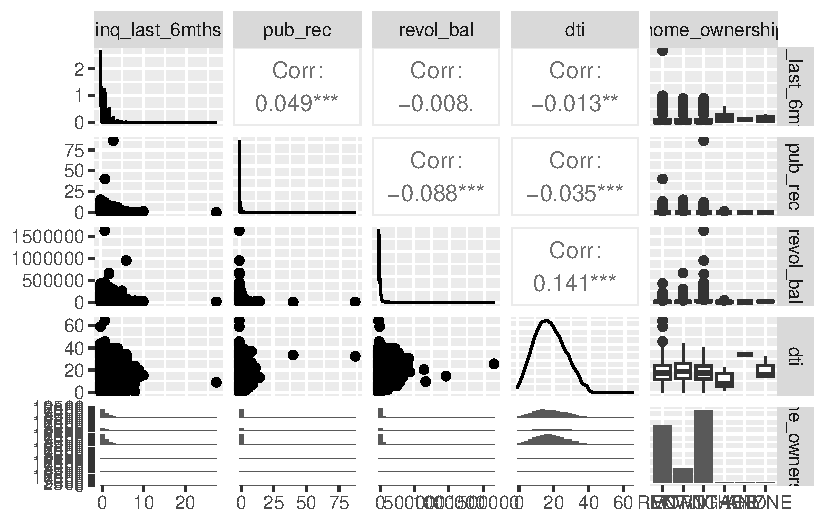
\includegraphics{P1-6-Haeusler_files/figure-pdf/unnamed-chunk-6-1.pdf}

}

\end{figure}

\begin{Shaded}
\begin{Highlighting}[]
\NormalTok{myLCdata\_clean }\OtherTok{\textless{}{-}} \FunctionTok{na.omit}\NormalTok{(myLCdata[, }\FunctionTok{c}\NormalTok{(}\StringTok{"inq\_last\_6mths"}\NormalTok{, }\StringTok{"pub\_rec"}\NormalTok{, }\StringTok{"revol\_bal"}\NormalTok{, }\StringTok{"dti"}\NormalTok{, }\StringTok{"home\_ownership"}\NormalTok{)])}
\CommentTok{\#ggpairs(myLCdata\_clean)}

\FunctionTok{suppressMessages}\NormalTok{(\{}
  \FunctionTok{ggpairs}\NormalTok{(myLCdata\_clean[, }\FunctionTok{c}\NormalTok{(}\StringTok{"inq\_last\_6mths"}\NormalTok{, }\StringTok{"pub\_rec"}\NormalTok{, }\StringTok{"revol\_bal"}\NormalTok{, }\StringTok{"dti"}\NormalTok{, }\StringTok{"home\_ownership"}\NormalTok{)])}
\NormalTok{\})}
\end{Highlighting}
\end{Shaded}

\begin{figure}[H]

{\centering 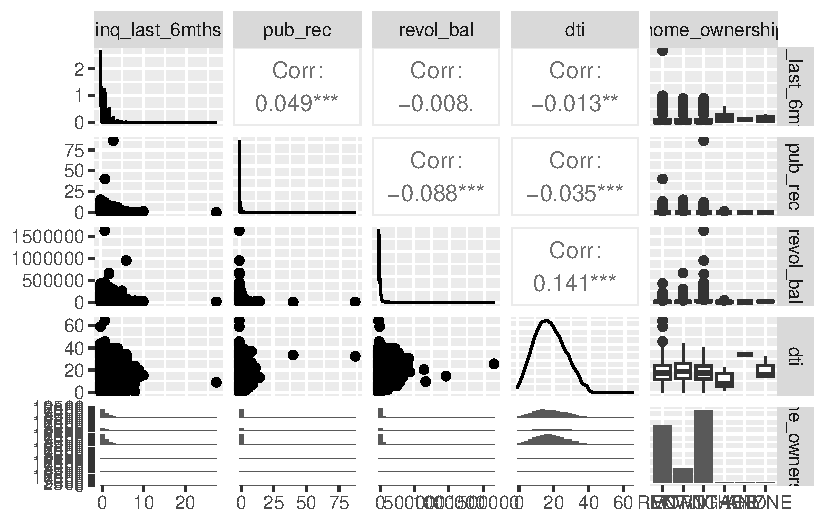
\includegraphics{P1-6-Haeusler_files/figure-pdf/unnamed-chunk-6-2.pdf}

}

\end{figure}

\begin{Shaded}
\begin{Highlighting}[]
\CommentTok{\# Create a box plot of revol\_bal grouped by home\_ownership}
\FunctionTok{boxplot}\NormalTok{(revol\_bal }\SpecialCharTok{\textasciitilde{}}\NormalTok{ home\_ownership, }\AttributeTok{data =}\NormalTok{ myLCdata,}
        \AttributeTok{main =} \StringTok{"Boxplot of Revolving Balance by Home Ownership"}\NormalTok{,}
        \AttributeTok{xlab =} \StringTok{"Home Ownership"}\NormalTok{,}
        \AttributeTok{ylab =} \StringTok{"Revolving Balance"}\NormalTok{,}
        \AttributeTok{col =} \StringTok{"skyblue"}\NormalTok{)}
\end{Highlighting}
\end{Shaded}

\begin{figure}[H]

{\centering \includegraphics{P1-6-Haeusler_files/figure-pdf/unnamed-chunk-7-1.pdf}

}

\end{figure}

\begin{Shaded}
\begin{Highlighting}[]
\CommentTok{\# Calculate the correlation between revol\_bal and dti}
\NormalTok{correlation }\OtherTok{\textless{}{-}} \FunctionTok{cor}\NormalTok{(myLCdata}\SpecialCharTok{$}\NormalTok{revol\_bal, myLCdata}\SpecialCharTok{$}\NormalTok{dti)}

\CommentTok{\# Create a scatterplot of dti against revol\_bal}
\FunctionTok{plot}\NormalTok{(myLCdata}\SpecialCharTok{$}\NormalTok{dti, myLCdata}\SpecialCharTok{$}\NormalTok{revol\_bal,}
     \AttributeTok{main =} \StringTok{"Scatterplot of Debt{-}to{-}Income Ratio vs. Revolving Balance"}\NormalTok{,}
     \AttributeTok{sub =} \FunctionTok{paste}\NormalTok{(}\StringTok{"Correlation ="}\NormalTok{, }\FunctionTok{round}\NormalTok{(correlation, }\DecValTok{2}\NormalTok{)),}
     \AttributeTok{xlab =} \StringTok{"Debt{-}to{-}Income Ratio"}\NormalTok{,}
     \AttributeTok{ylab =} \StringTok{"Revolving Balance"}\NormalTok{,}
     \AttributeTok{col =} \StringTok{"blue"}\NormalTok{)}

\CommentTok{\# Add correlation coefficient to the plot}
\FunctionTok{text}\NormalTok{(}\AttributeTok{x =} \FunctionTok{min}\NormalTok{(myLCdata}\SpecialCharTok{$}\NormalTok{dti), }
     \AttributeTok{y =} \FunctionTok{max}\NormalTok{(myLCdata}\SpecialCharTok{$}\NormalTok{revol\_bal),}
     \AttributeTok{labels =} \FunctionTok{paste}\NormalTok{(}\StringTok{"Correlation ="}\NormalTok{, }\FunctionTok{round}\NormalTok{(correlation, }\DecValTok{2}\NormalTok{)),}
     \AttributeTok{pos =} \DecValTok{4}\NormalTok{, }\AttributeTok{cex =} \FloatTok{0.8}\NormalTok{, }\AttributeTok{col =} \StringTok{"black"}\NormalTok{)}
\end{Highlighting}
\end{Shaded}

\begin{figure}[H]

{\centering \includegraphics{P1-6-Haeusler_files/figure-pdf/unnamed-chunk-7-2.pdf}

}

\end{figure}

\begin{Shaded}
\begin{Highlighting}[]
\CommentTok{\# Exclude rows with missing values in inq\_last\_6mths and pub\_rec}
\NormalTok{complete\_cases }\OtherTok{\textless{}{-}} \FunctionTok{complete.cases}\NormalTok{(myLCdata}\SpecialCharTok{$}\NormalTok{inq\_last\_6mths, myLCdata}\SpecialCharTok{$}\NormalTok{pub\_rec)}
\NormalTok{inq\_last\_6mths }\OtherTok{\textless{}{-}}\NormalTok{ myLCdata}\SpecialCharTok{$}\NormalTok{inq\_last\_6mths[complete\_cases]}
\NormalTok{pub\_rec }\OtherTok{\textless{}{-}}\NormalTok{ myLCdata}\SpecialCharTok{$}\NormalTok{pub\_rec[complete\_cases]}

\CommentTok{\# Calculate the correlation between inq\_last\_6mths and pub\_rec}
\NormalTok{correlation\_2 }\OtherTok{\textless{}{-}} \FunctionTok{cor}\NormalTok{(inq\_last\_6mths, pub\_rec)}

\CommentTok{\# Create a scatterplot of pub\_rec against inq\_last\_6mths}
\FunctionTok{plot}\NormalTok{(inq\_last\_6mths, pub\_rec,}
     \AttributeTok{main =} \StringTok{"Scatterplot of Inquiries in Last 6 Months vs. Public Records"}\NormalTok{,}
     \AttributeTok{sub =} \FunctionTok{paste}\NormalTok{(}\StringTok{"Correlation ="}\NormalTok{, }\FunctionTok{round}\NormalTok{(correlation\_2, }\DecValTok{2}\NormalTok{)),}
     \AttributeTok{xlab =} \StringTok{"Inquiries in Last 6 Months"}\NormalTok{,}
     \AttributeTok{ylab =} \StringTok{"Public Records"}\NormalTok{,}
     \AttributeTok{col =} \StringTok{"blue"}\NormalTok{)}
\end{Highlighting}
\end{Shaded}

\begin{figure}[H]

{\centering \includegraphics{P1-6-Haeusler_files/figure-pdf/unnamed-chunk-7-3.pdf}

}

\end{figure}

\begin{Shaded}
\begin{Highlighting}[]
\CommentTok{\# Exclude rows with missing values in dti and inq\_last\_6mths}
\NormalTok{complete\_cases }\OtherTok{\textless{}{-}} \FunctionTok{complete.cases}\NormalTok{(myLCdata}\SpecialCharTok{$}\NormalTok{dti, myLCdata}\SpecialCharTok{$}\NormalTok{inq\_last\_6mths)}
\NormalTok{dti }\OtherTok{\textless{}{-}}\NormalTok{ myLCdata}\SpecialCharTok{$}\NormalTok{dti[complete\_cases]}
\NormalTok{inq\_last\_6mths }\OtherTok{\textless{}{-}}\NormalTok{ myLCdata}\SpecialCharTok{$}\NormalTok{inq\_last\_6mths[complete\_cases]}

\CommentTok{\# Calculate the correlation between dti and inq\_last\_6mths}
\NormalTok{correlation\_3 }\OtherTok{\textless{}{-}} \FunctionTok{cor}\NormalTok{(dti, inq\_last\_6mths)}

\CommentTok{\# Create a scatterplot of dti against inq\_last\_6mths}
\FunctionTok{plot}\NormalTok{(inq\_last\_6mths, dti,}
     \AttributeTok{main =} \StringTok{"Scatterplot of Debt{-}to{-}Income Ratio vs. Inquiries in Last 6 Months"}\NormalTok{,}
     \AttributeTok{sub =} \FunctionTok{paste}\NormalTok{(}\StringTok{"Correlation ="}\NormalTok{, }\FunctionTok{round}\NormalTok{(correlation\_3, }\DecValTok{2}\NormalTok{)),}
     \AttributeTok{xlab =} \StringTok{"Inquiries in Last 6 Months"}\NormalTok{,}
     \AttributeTok{ylab =} \StringTok{"Debt{-}to{-}Income Ratio"}\NormalTok{,}
     \AttributeTok{col =} \StringTok{"blue"}\NormalTok{)}
\end{Highlighting}
\end{Shaded}

\begin{figure}[H]

{\centering \includegraphics{P1-6-Haeusler_files/figure-pdf/unnamed-chunk-7-4.pdf}

}

\end{figure}

\begin{Shaded}
\begin{Highlighting}[]
\CommentTok{\# Convert home\_ownership to factor if it\textquotesingle{}s not already}
\NormalTok{myLCdata}\SpecialCharTok{$}\NormalTok{home\_ownership }\OtherTok{\textless{}{-}} \FunctionTok{factor}\NormalTok{(myLCdata}\SpecialCharTok{$}\NormalTok{home\_ownership)}

\CommentTok{\# Create a matrix of scatterplots}
\FunctionTok{pairs}\NormalTok{(}\SpecialCharTok{\textasciitilde{}}\NormalTok{ inq\_last\_6mths }\SpecialCharTok{+}\NormalTok{ pub\_rec }\SpecialCharTok{+}\NormalTok{ revol\_bal }\SpecialCharTok{+}\NormalTok{ dti }\SpecialCharTok{+}\NormalTok{ home\_ownership, }\AttributeTok{data =}\NormalTok{ myLCdata,}
      \AttributeTok{main =} \StringTok{"Scatterplot Matrix"}\NormalTok{)}
\end{Highlighting}
\end{Shaded}

\begin{figure}[H]

{\centering 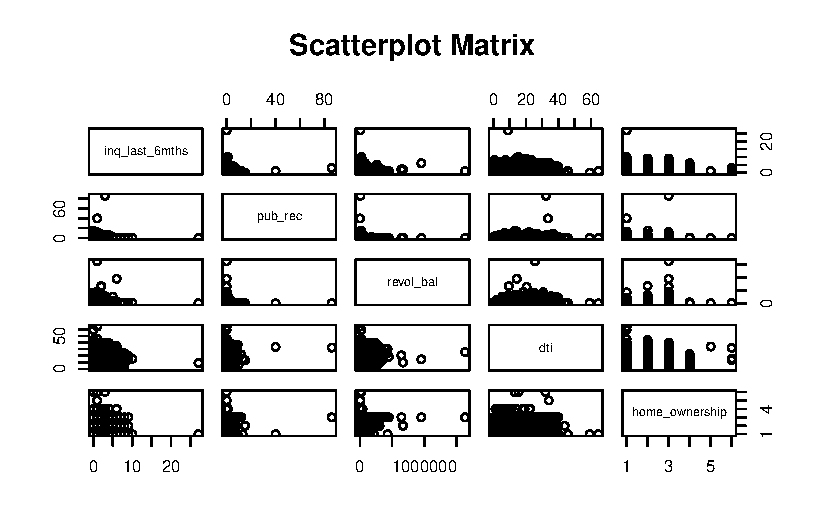
\includegraphics{P1-6-Haeusler_files/figure-pdf/unnamed-chunk-7-5.pdf}

}

\end{figure}

\textbf{Add Text}

\begin{Shaded}
\begin{Highlighting}[]
\FunctionTok{library}\NormalTok{(dplyr)}
\FunctionTok{library}\NormalTok{(ggplot2)}

\CommentTok{\# Remove missing values from revol\_bal and inq\_last\_6mths variables}
\NormalTok{cleaned\_data }\OtherTok{\textless{}{-}}\NormalTok{ myLCdata }\SpecialCharTok{\%\textgreater{}\%}
  \FunctionTok{filter}\NormalTok{(}\SpecialCharTok{!}\FunctionTok{is.na}\NormalTok{(revol\_bal), }\SpecialCharTok{!}\FunctionTok{is.na}\NormalTok{(inq\_last\_6mths)) }\SpecialCharTok{\%\textgreater{}\%}
  \FunctionTok{filter}\NormalTok{(}
\NormalTok{    revol\_bal }\SpecialCharTok{\textless{}} \FunctionTok{quantile}\NormalTok{(revol\_bal, }\FloatTok{0.99}\NormalTok{, }\AttributeTok{na.rm =} \ConstantTok{TRUE}\NormalTok{) }\SpecialCharTok{\&} 
\NormalTok{    inq\_last\_6mths }\SpecialCharTok{\textless{}} \FunctionTok{quantile}\NormalTok{(inq\_last\_6mths, }\FloatTok{0.99}\NormalTok{, }\AttributeTok{na.rm =} \ConstantTok{TRUE}\NormalTok{)}
\NormalTok{  )}

\CommentTok{\# Create scatterplot}
\FunctionTok{ggplot}\NormalTok{(cleaned\_data, }\FunctionTok{aes}\NormalTok{(}\AttributeTok{x =}\NormalTok{ revol\_bal, }\AttributeTok{y =}\NormalTok{ inq\_last\_6mths)) }\SpecialCharTok{+}
  \FunctionTok{geom\_point}\NormalTok{() }\SpecialCharTok{+}
  \FunctionTok{labs}\NormalTok{(}\AttributeTok{title =} \StringTok{"Scatterplot of Revolving Balance vs. Inquiries in Last 6 Months"}\NormalTok{,}
       \AttributeTok{x =} \StringTok{"Revolving Balance"}\NormalTok{,}
       \AttributeTok{y =} \StringTok{"Inquiries in Last 6 Months"}\NormalTok{)}
\end{Highlighting}
\end{Shaded}

\begin{figure}[H]

{\centering \includegraphics{P1-6-Haeusler_files/figure-pdf/unnamed-chunk-8-1.pdf}

}

\end{figure}

\begin{Shaded}
\begin{Highlighting}[]
\CommentTok{\# Select only numeric variables from myLCdata}
\NormalTok{numeric\_data }\OtherTok{\textless{}{-}}\NormalTok{ myLCdata[, }\FunctionTok{sapply}\NormalTok{(myLCdata, is.numeric)]}

\CommentTok{\# Remove missing values}
\NormalTok{numeric\_data\_noNA }\OtherTok{\textless{}{-}} \FunctionTok{na.omit}\NormalTok{(numeric\_data)}

\CommentTok{\# Convert data frame to matrix{-}like object}
\NormalTok{numeric\_matrix }\OtherTok{\textless{}{-}} \FunctionTok{as.matrix}\NormalTok{(numeric\_data\_noNA)}

\CommentTok{\# Calculate correlation matrix}
\NormalTok{correlation\_matrix }\OtherTok{\textless{}{-}} \FunctionTok{cor}\NormalTok{(numeric\_matrix)}

\CommentTok{\# Print correlation matrix}
\FunctionTok{print}\NormalTok{(correlation\_matrix)}
\end{Highlighting}
\end{Shaded}

\begin{verbatim}
     [,1]
[1,]    1
\end{verbatim}



\end{document}
